%課題研究レジュメテンプレート ver. 1.2

\documentclass[uplatex]{jsarticle}
\usepackage[top=20mm,bottom=20mm,left=20mm,right=20mm]{geometry}
\usepackage[T1]{fontenc}
\usepackage{txfonts}
\usepackage{wrapfig}
\usepackage[expert,deluxe]{otf}
\usepackage[dvipdfmx,hiresbb]{graphicx}
\usepackage[dvipdfmx]{hyperref}
\usepackage{pxjahyper}
\usepackage{secdot}
\usepackage{float}

\makeatletter
  \renewcommand{\section}{%
    \if@slide\clearpage\fi
    \@startsection{section}{1}{\z@}%
    {\Cvs \@plus.5\Cdp \@minus.2\Cdp}% 前アキ
    {.5\Cvs \@plus.3\Cdp}% 後アキ
    %{\normalfont\Large\headfont\raggedright}}
    {\normalfont\raggedright}}

  \renewcommand{\subsection}{\@startsection{subsection}{2}{\z@}%
    {\Cvs \@plus.5\Cdp \@minus.2\Cdp}% 前アキ
    {.5\Cvs \@plus.3\Cdp}% 後アキ
    %{\normalfont\large\headfont}}
    {\normalfont}}

  \renewcommand{\subsubsection}{\@startsection{subsubsection}{3}{\z@}%
    {\Cvs \@plus.5\Cdp \@minus.2\Cdp}%
    {\z@}%
    %{\normalfont\normalsize\headfont}}
    {\normalfont}}
\makeatother
%ここから上を編集する必要はない.





\title{\vspace{-14mm}クラウドファンディングにおける金額の推移の調査}
\author{PMコース 矢吹研究室 1342066 氏名 島田 樹}
\date{}%日付を入れる必要はない.
\pagestyle{empty}%ページ番号は振らない.
\begin{document}
\maketitle





\section{研究の背景}

近年クラウドファンディングを利用したプロジェクトがSNSを発達に伴い年々増加しており,ニュースでも報じられるようになった.SNSの発達に伴いプロジェクトの数が年々増加している.
クラウドファンディングとはプロジェクトの必要資金を,インターネットを利用し,不特定多数の支援者から資金提供を募集する資金調達の手法である.大手企業から個人のプロジェクトまで幅広い規模のプロジェクトで応募が可能であり,近年ベンチャー企業や学生にチャンスを与えるものとして注目を集めている.クラウドファンディングは一般的に資金提供者に対するリターンの形態によって以下の3つに分けることができる\cite{crwowd}.
\begin{enumerate}
 \item 金銭的リターンのない「寄付型」
 \item 金銭的リターンのある「投資型」
 \item 権利や物品を購入することで支援する「購入型」
\end{enumerate}
日本では金融商品取引法の規制などの関係上,購入型が最も普及しており,アメリカのKickstarter\cite{kickstarter}をはじめ,日本のCAMPFIRE\cite{camp}やREADYFOR\cite{readyfor}も購入型になる.今回は日本で最初のクラウドファンディングサイトであるREADYFORと,Makuake\cite{makuake}で掲載されているプロジェクトの金額の推移を調査する.




\section{研究の目的}

READYFORとMakuakeで掲載されているプロジェクトから,1日ごとの金額データを集めてグラフにする.グラフを分類し金額の推移のパターンを明らかにする.




\section{プロジェクトマネジメントとの関連}

クラウドファンディングの金額の推移のパターンを明らかにすることで,プロジェクトの傾向がつかめる.これにより資金集めの段階で成功率を上げられると考えられる.




\section{研究の方法}

以下の手順で研究を行った.
\begin{enumerate}
 \item READYFORと,Makuakeのプロジェクトの中から監視するプロジェクトを選定する.
 \item 毎日同じ時間にプロジェクトのウェブページを保存し,金額の推移を記録する.
 \item プロジェクトの終了までの金額の推移をグラフにする.
 \item グラフの形から種類を分類する.
\end{enumerate}


\section{現在の進捗状況}

%\begin{wrapfigure}[行数]{r}{幅}%行数はオプションだが,調整しないとうまくいかない.
\begin{wrapfigure}[11]{H}{13cm}
\vspace*{-\intextsep}
%\includegraphics[width=図の幅,clip]{ファイル名}\label{参照用ラベル}
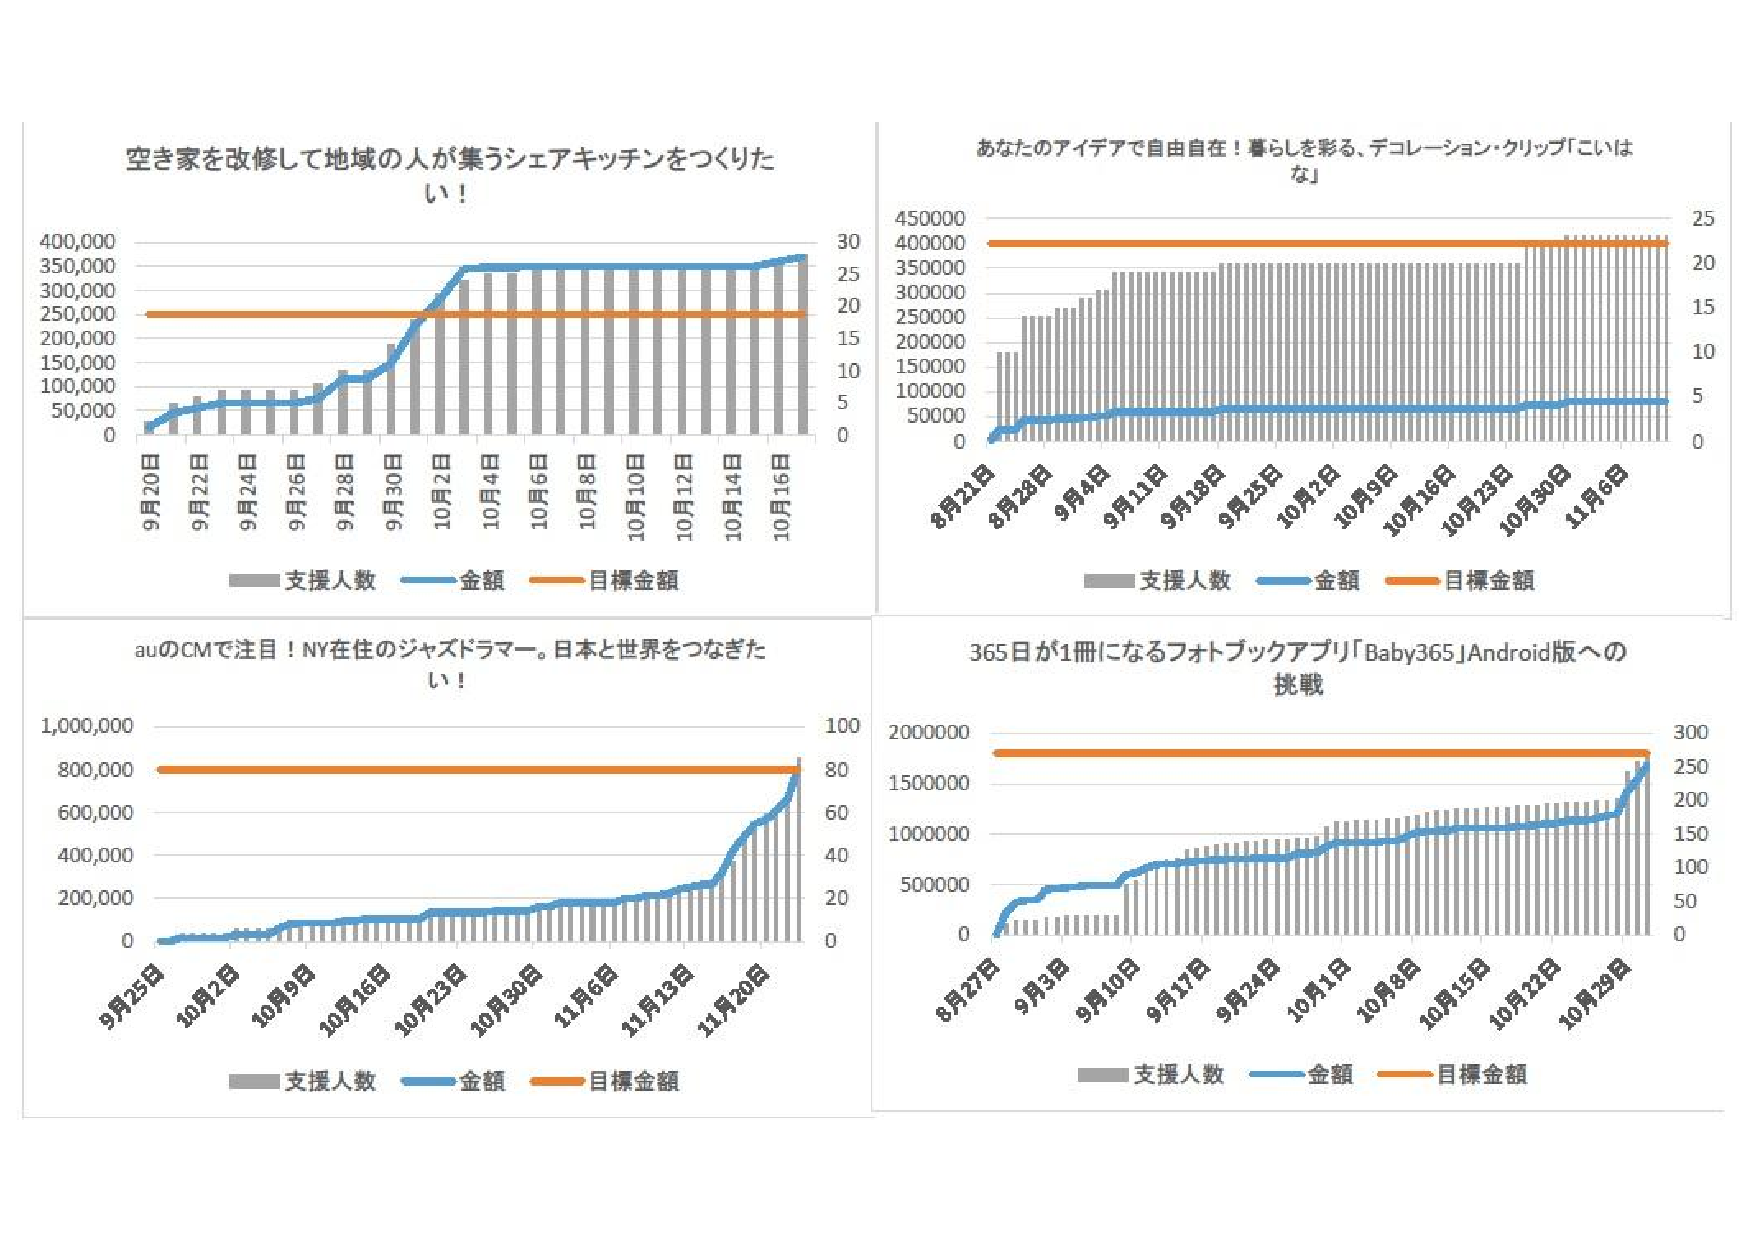
\includegraphics[width=10cm,clip]{images.pdf}
\caption{金額の推移}\label{サンプル図}
\end{wrapfigure}


\subsection{結果}
集めたデータからグラフを作成し分類したところ,4種類に分類された.成功と失敗で大きく二つに分類し,さらにプロジェクト終了間際に特徴的な動きをしたものを分類した.グラフの結果から終了直前の金額が大きく推移しているプロジェクトがあることがわかる.
\subsection{考察}
終了直前の金額が大きく推移している理由として,終了直前にそのプロジェクトが成功するかどうか確認する人が多いと考えられる.その中で成功に至ったプロジェクトは,直前に成功する見込みがあると判断されたと言える.




\section{今後の計画}
今後はさらに多くのプロジェクトからデータを取り結果の精度を上げるとともに,終了直前での金額の伸びに着目し,その要因を見つけることを目標とする.
以下のように研究を進める計画である.

\begin{enumerate}
\item データを自動で集められるように環境を整える. 
\item データを集めるサイトを増やす.
\item 金額の推移に関わっている要因を探す.
\end{enumerate}

\bibliographystyle{junsrt}
\bibliography{biblio}%「biblio.bib」というファイルが必要.

\end{document}
